\svnkwsave{$RepoFile: siminos/baroclinic/dailyBlog.tex $}
\svnidlong {$HeadURL$}
{$LastChangedDate$}
{$LastChangedRevision$} {$LastChangedBy$}
\svnid{$Id$}

\chapter{Blog}
\label{chap:dailyBlog}

\begin{bartlett}{
I am usually as happy as possible in any situation.
}
\bauthor{
Joe
    }
\end{bartlett}


\section{Daily blog, point by point}
\label{sect:blogBaroclin}

%%%%%%%%%%%%%%%%%%%%%%%%%%%%%%%%%%%%%%%%%%%%%%%%%%%%%%%%%%%%%%%%%%%%%
\FIG{
 (a)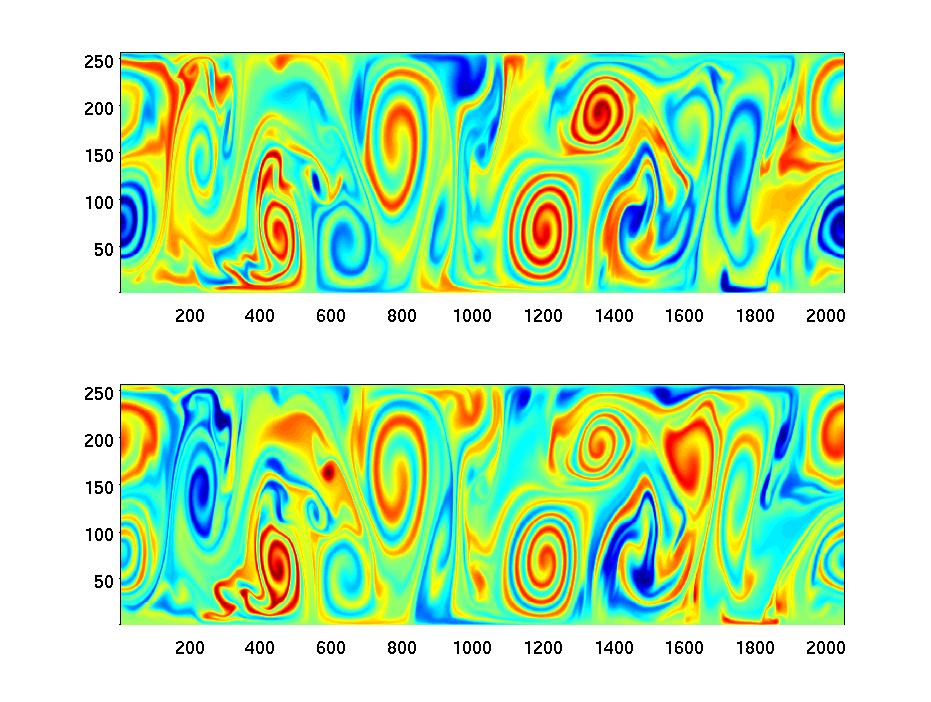
\includegraphics[width=0.85\textwidth]{111018t32_NL}
\\
(b)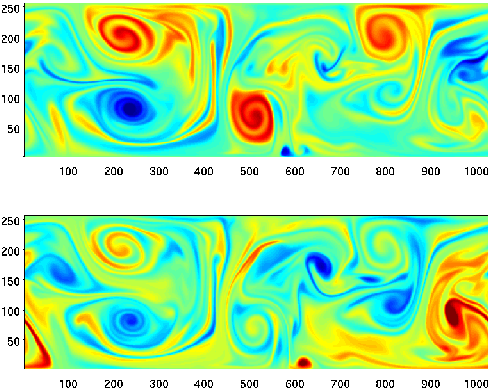
\includegraphics[width=0.85\textwidth]{111018reduced}
 }{}{
2 layers: top, bottom.
(a)
The usual domain $L=8$.
(b)
The reduced domain $L=4$, initial conditions starting
from a linear solution. The energy is not yet fully equilibrated.
The longer
cell (a) behaves pretty much the same way, but overall
the circulation is a bit stronger.
}{2layerBclin}
%%%%%%%%%%%%%%%%%%%%%%%%%%%%%%%%%%%%%%%%%%%%%%%%%%%%%%%%%%%%%%%%%%%%%

\begin{description}

\item[2011-05-27 Predrag, weather report from Snowbird DS11]
	\toCB
Learned from Pierrehumbert that the baroclinic models are to weathermen
what ``harmonic oscillator'' is to quantum mechanics. It has a continuous
East-West translational symmetry, \ie, in a periodic box it needs to be
sliced (the \SOn{2} of periodic box quotiented out).

Tried to proselytize Christian Wolfe\rf{WoSa07}, Scripts,  make him slice
the baroclinic instability, and, perchance, if I get him there, recycle
it, former Gibson style. Pierrehumbert says that this would be persuasive
to weather people, convince them to go looking for exact unstable
invariant solutions. After one hour Wolfe said he was converted.

Tried ditto with Pierrehumbert and Silber postdoc Yi-Ping Ma (Knobloch
trained, has worked with Spiegel at Woods Hole GFD). He does not know any
geophysical fluid dynamics yet, so I'm sceptical that he will do anything.

\item[2011-05-27 Annalisa Bracco]
If you ever need a code that produce baroclinic instability, I have
plenty. Worked with the Joe Pedlosky, the expert on Baroclinic
Instability, as a postdoc. I also have an easy atmospheric model (global,
on a sphere etc) that reproduces very well baroclinic instability as per
observations and can be run as aqua-planet to simplify things.

\item[2011-05-27 Predrag]
We could make Joe Pedlosky happy? Let's do it before August, in time for
Woods Hole. The first step is to slice your simulations for a minimal
periodic cell of interest (narrow but turbulent). The second step might
be either to determine ``physical dimension'' using
Wolfe-Samelson\rf{WoSa07} Lyapunov vectors (that is just simulation) or
find some traveling waves (that is Krylov-Arnoldi nontrivial work, but
for low-dimensional discretizations might be doable by Newton).

\item[2011-10-15 Annalisa]
Shown Predrag some simulations.
Each layer is computed in
terms of vorticity equations as a 2-dimensional fluid. The lower layer
has higher fluid density, and they are coupled across their interface by
difference of vorticity.
In our simulation this is about factor two; it is related to the
R\"osby deformation radius $L_R$. The spanwise $y$ width is $L_R/2\pi =
1/2$. Unless the width is larger than $L_R$, no instability. The
stream-wise aspect ration is about 8.
They tend to the barotropic solution (vortices rotating the same way on
top and bottom).


Discussion of solutions:
\begin{enumerate}
  \item [1)]
is linear: dropped the nonlinear term \ie\ the Jacobian of the vorticity
and the stream function. Instability is seeded by a small random field of
prescribed power spectrum, but the resulting instability is a localized
wave (about 3 rolls) with streamwise/spanwise ratio of about 1/2 set
$L_R$. That sets the scale of the instability off the laminar solution.
Initial noise does not matter, as the instability grows very fast. The
two layer vorticities are opposite.

  \item [2)] is fully nonlinear, all other parameters the same.

  \item [3)]
\end{enumerate}

\item[2011-10-18 Annalisa]

\refFig{2layerBclin}\,(a)
The usual domain $L=8$, 2 layers. Note that as for initial conditions,
the overall the flow is more energetic.

\refFig{2layerBclin}\,(b)
The reduced domain $L=4$, 2 layers. Correct initial conditions, starting
from a linear solution. The energy is not yet fully equilibrated. One
problem I can see is that the periodic boundary conditions may prevent
perfect equilibration. The longer cell \refFig{2layerBclin}\,(a) behaves
pretty much the same way, but overall the circulation is a bit stronger.

\item[2011-10-19 Annalisa]
There is a barotropization issue, likely due to the periodic boundaries.
My guess is that we'll not need a very long simulation and we can live
with a non perfectly stationary state, essentially the eddies that form
in the equilibrated solution prefer to be barotropic -same sign top and
bottom layer- because they are more stable and in the absence of
viscosity they are an exact solution of \NS, and the simulation goes
into a state that resembles the long-term state for 2-d turbulence. If we
could work only over times $\sim $40-70 we should be all set.

For now the time is just in code units, I'll convert it in something
meaningful once we decide on which run to use, \etc.

%%%%%%%%%%%%%%%%%%%%%%%%%%%%%%%%%%%%%%%%%%%%%%%%%%%%%%%%%%%%%%%%%%%%%
\begin{figure}[t]
\begin{center}
% \begin{tabular}{cc}
%        ~~~~~~~~(\textit{a})                        &   ~~~~~~~~(\textit{b}) \\
    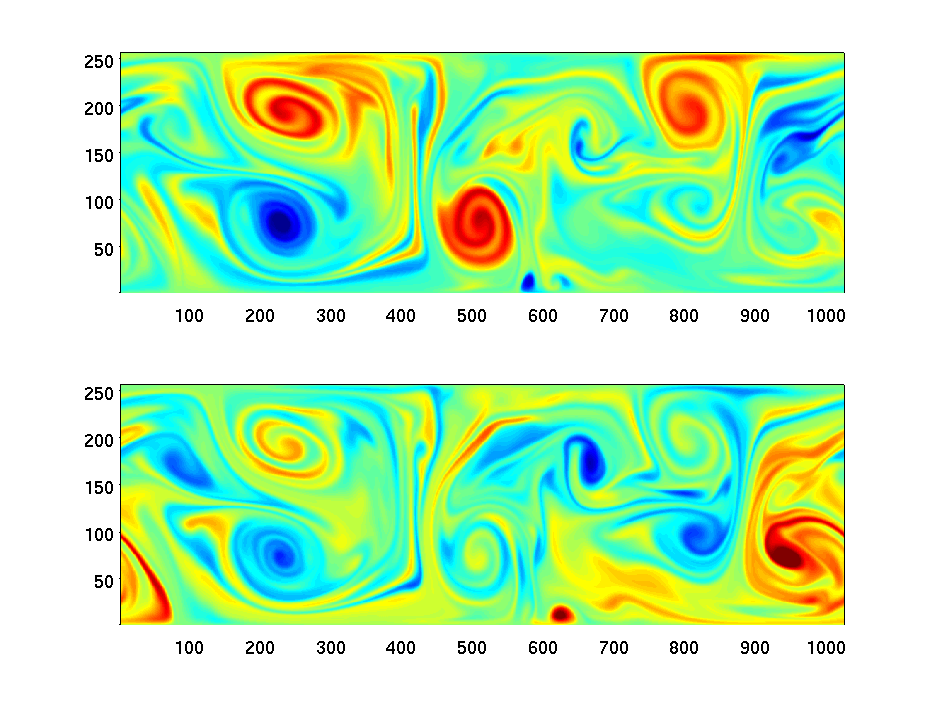
\includegraphics[width=0.95\textwidth]{111018time50}
%    &
    \\
    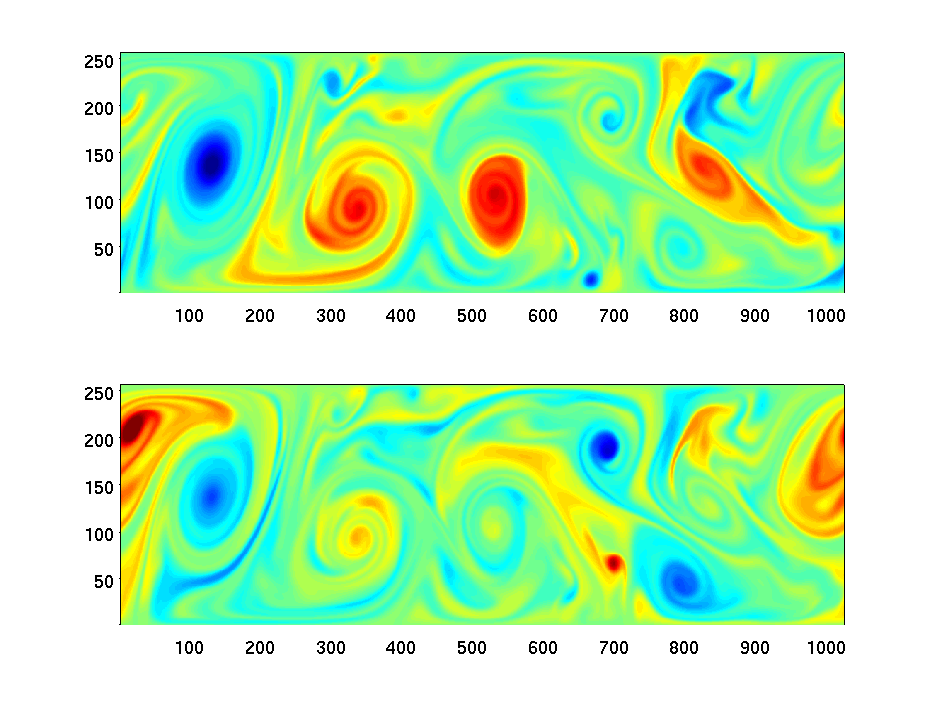
\includegraphics[width=0.95\textwidth]{111018time70}
%  \end{tabular}
\end{center}
\caption{
A plot of the vorticity in the top/bottom layers at times 50 and 70.
        }
\label{f:111018time1}
\end{figure}
%%%%%%%%%%%%%%%%%%%%%%%%%%%%%%%%%%%%%%%%%%%%%%%%%%%%%%%%%%%%%%%%%%%%%

%%%%%%%%%%%%%%%%%%%%%%%%%%%%%%%%%%%%%%%%%%%%%%%%%%%%%%%%%%%%%%%%%%%%%
\begin{figure}[t]
\begin{center}
% \begin{tabular}{cc}
%        ~~~~~~~~(\textit{a})                        &   ~~~~~~~~(\textit{b}) \\
    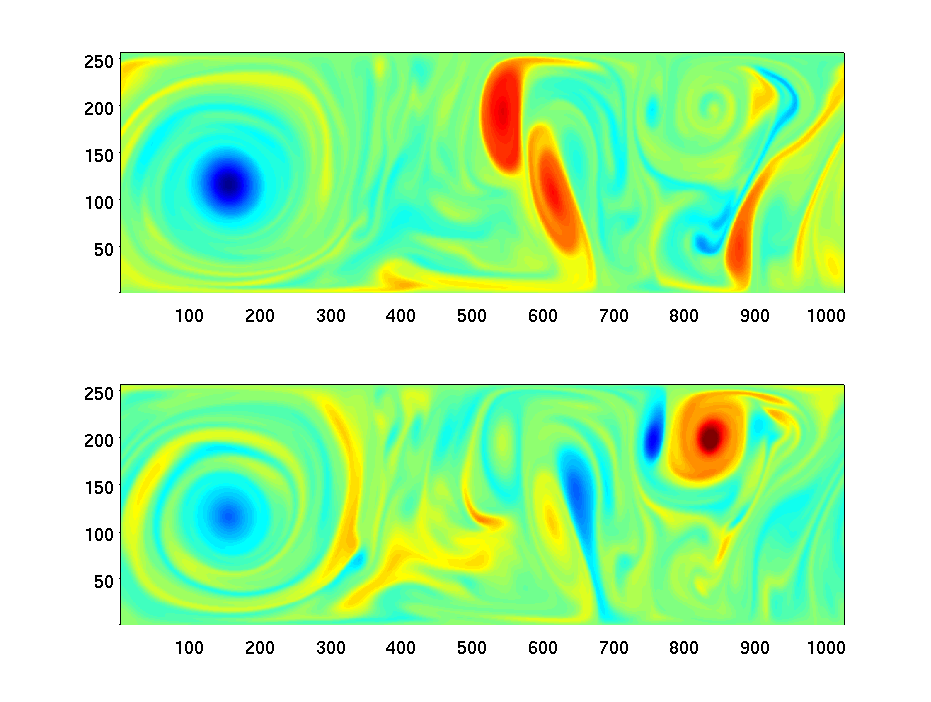
\includegraphics[width=0.95\textwidth]{111018time100}
%    &
%    \\
%    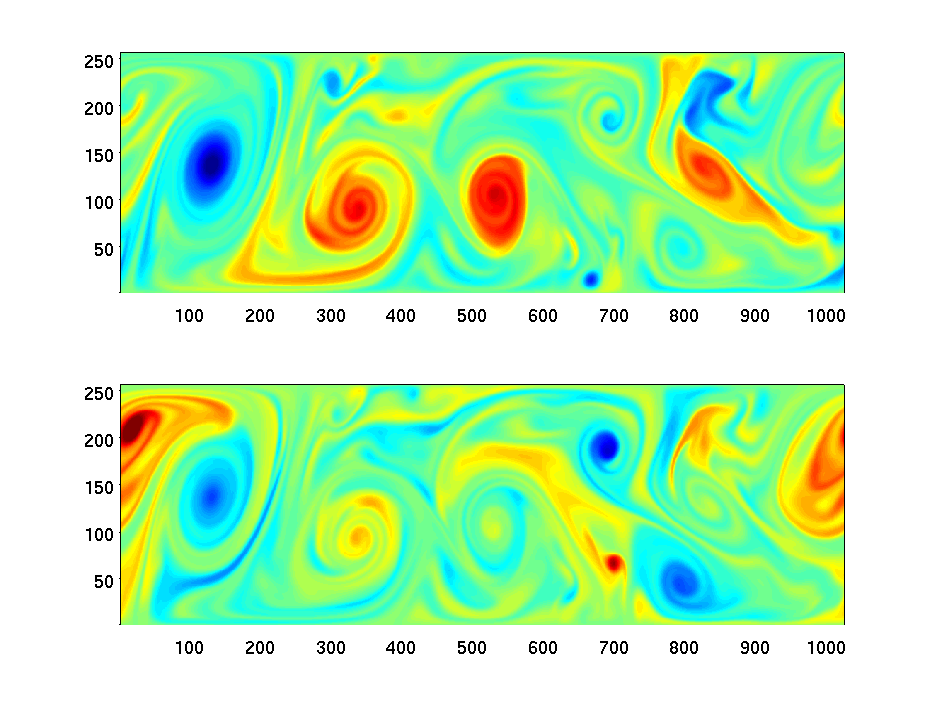
\includegraphics[width=0.95\textwidth]{111018time70}
%  \end{tabular}
\end{center}
\caption{
A plot of the vorticity in the top/bottom layers at time 100.
        }
\label{f:111018time2}
\end{figure}
%%%%%%%%%%%%%%%%%%%%%%%%%%%%%%%%%%%%%%%%%%%%%%%%%%%%%%%%%%%%%%%%%%%%%

%%%%%%%%%%%%%%%%%%%%%%%%%%%%%%%%%%%%%%%%%%%%%%%%%%%%%%%%%%%%%%%%%%%%%
\begin{figure}[t]
\begin{center}
% \begin{tabular}{cc}
%        ~~~~~~~~(\textit{a})                        &   ~~~~~~~~(\textit{b}) \\
    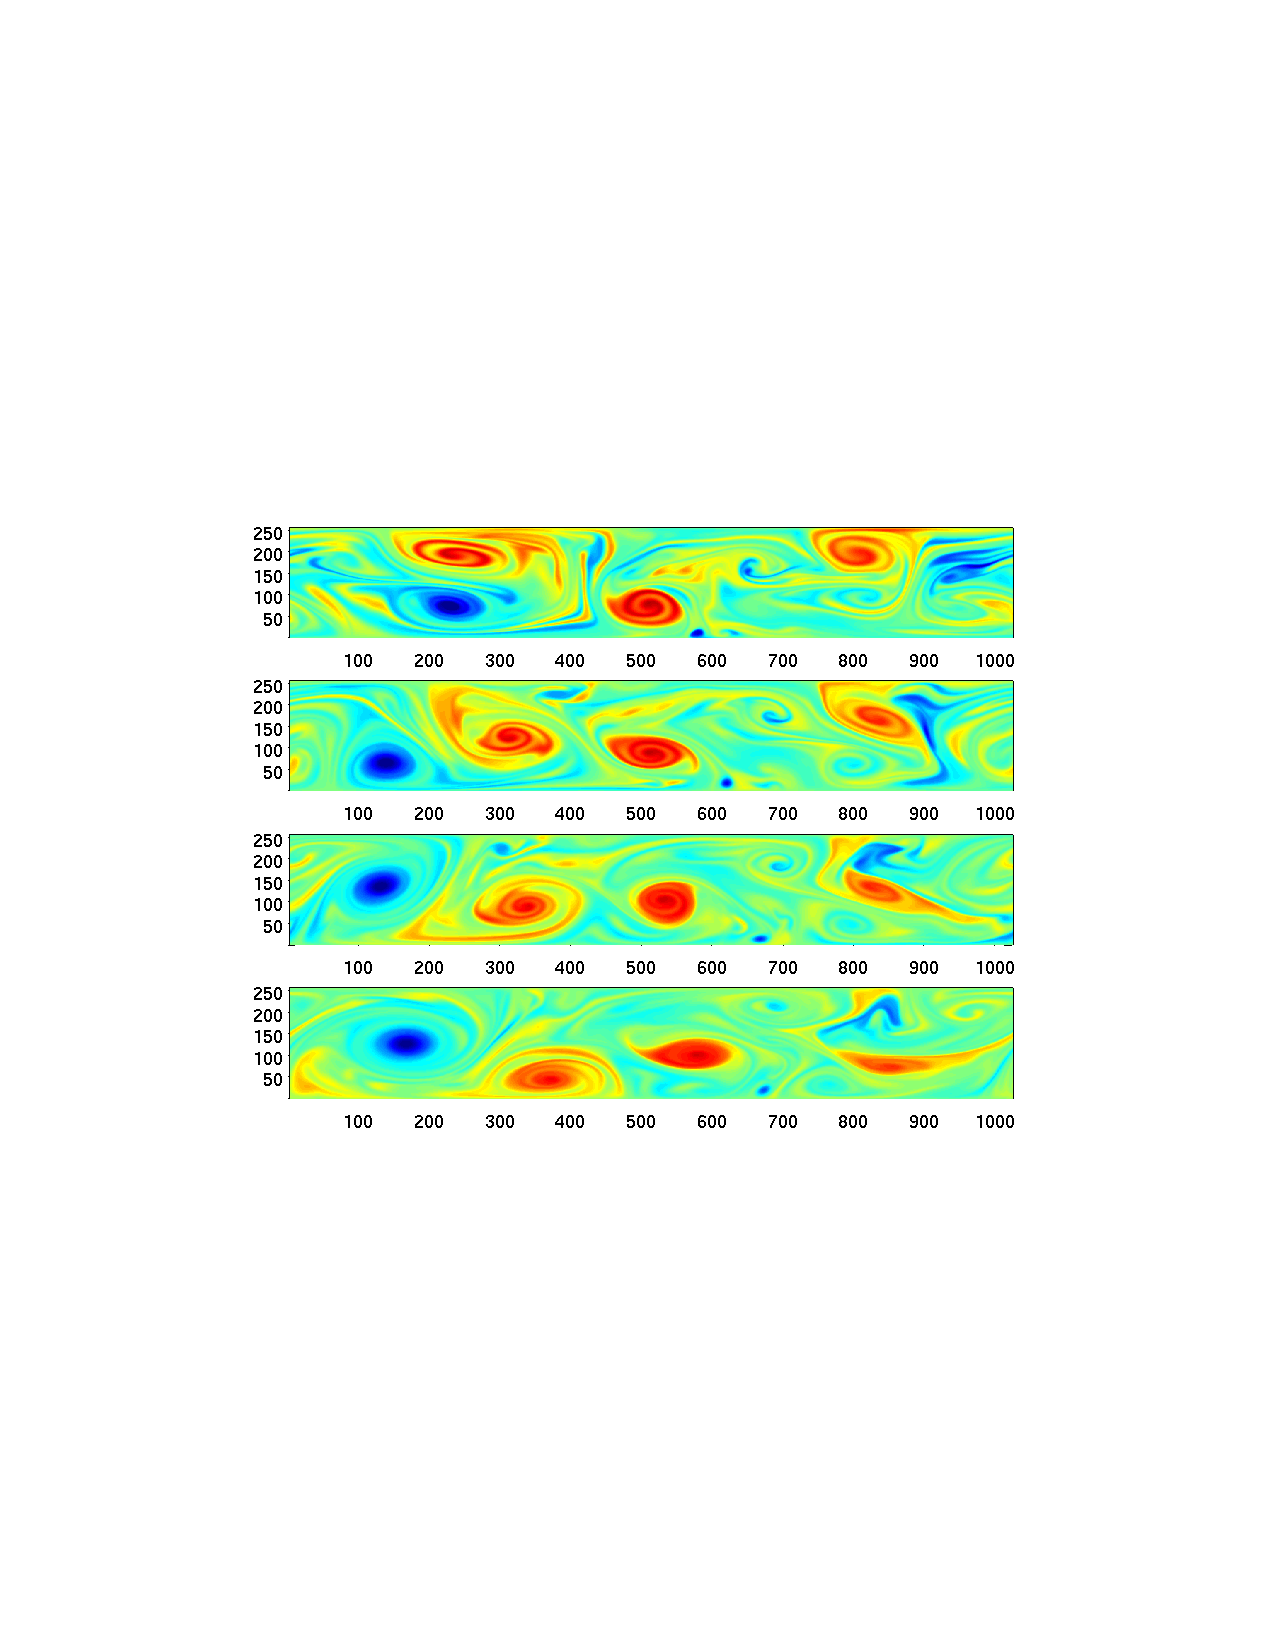
\includegraphics[width=0.95\textwidth]{111024layer1}
%    & 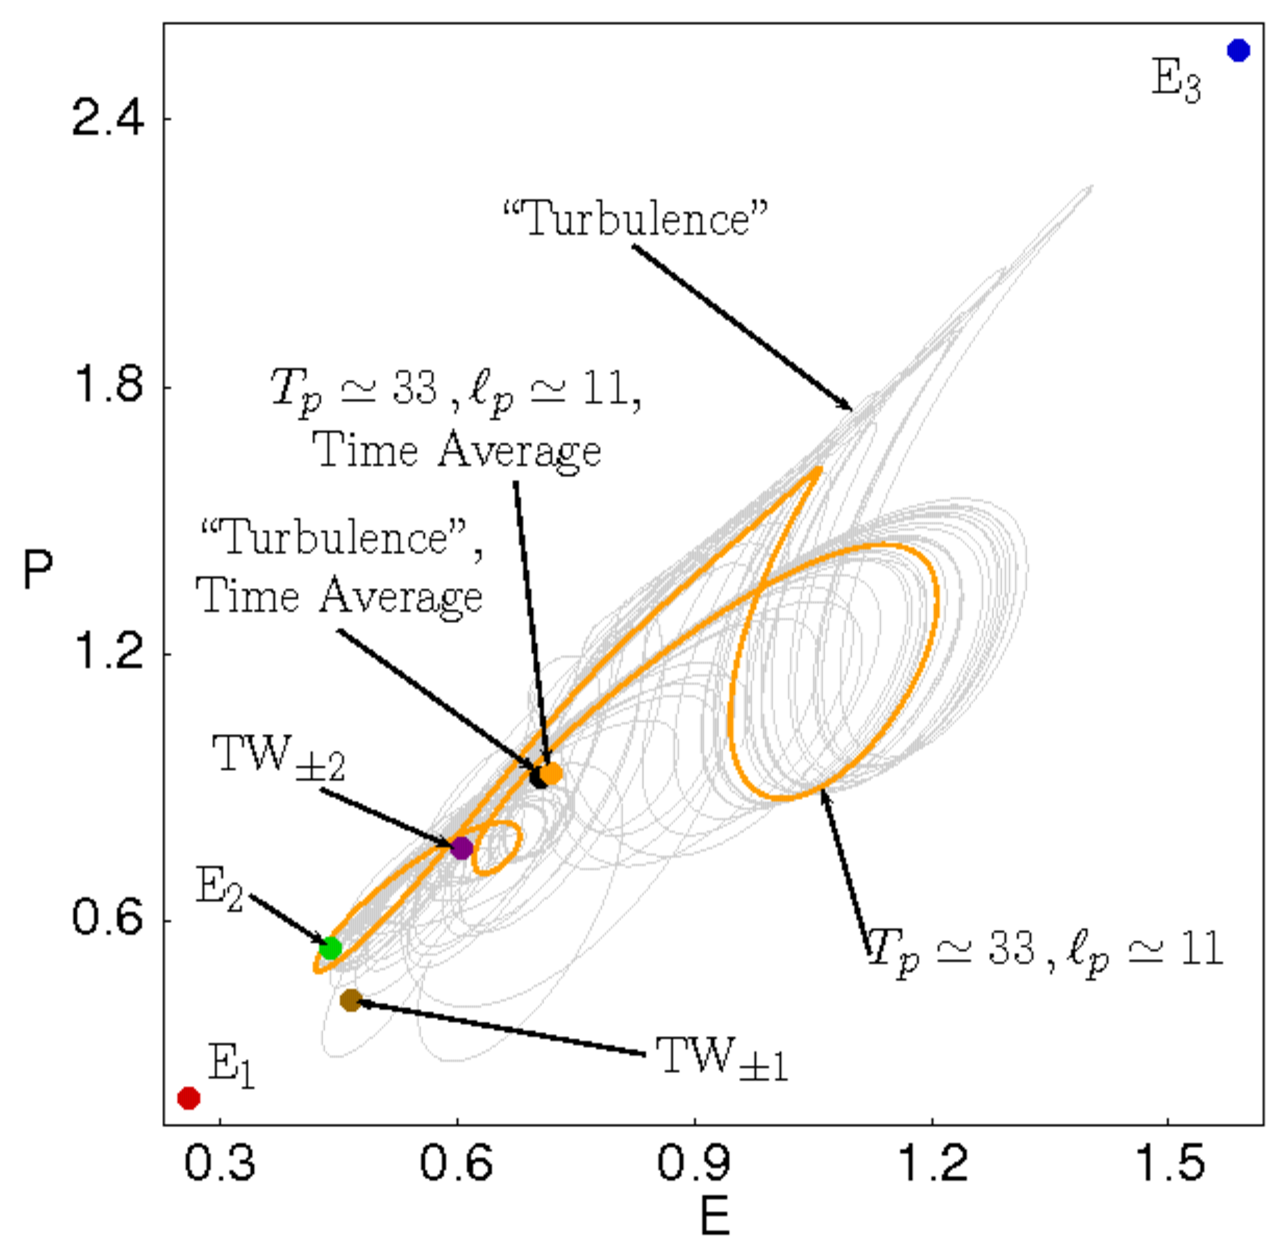
\includegraphics[width=0.46\textwidth, clip=true]{equivaEP_pst}
%  \end{tabular}
\end{center}
\caption{
A plot of the vorticity in the top layer at 4 different times during
which the energy is $\approx$ stable. The structures remain the same,
they are just moving a bit.
        }
\label{f:111024layer1}
\end{figure}
%%%%%%%%%%%%%%%%%%%%%%%%%%%%%%%%%%%%%%%%%%%%%%%%%%%%%%%%%%%%%%%%%%%%%



\item[2011-10-20 Predrag]
Bit worried if we are in transient turbulence, on the way to a
barotropic state, but might work out...

\item[2011-10-20 Annalisa]
One way to reduce the problem may be to stick to the 'longer' domain.
Another is to introduce a sponge region on one side. It will not solve the problem
completely: eddies are just more stable if barotropic and they tend to
become so while equilibrating a baroclinic solution, but it may delay
it.

\item[2011-10-20 Predrag]
It's OK that whole thing decays to barotropic, as long as we can find
unstable equilibrium solutions. Next (big) step. The short step is
to start looking at the dynamics of a short domain in the state space,
as explained in ChaosBook.org/tutorials, click on 'state space' in the
menu on the left.

\item[2011-10-20 Annalisa]
I may be able to stabilize it in a weakly nonlinear regime without
vortices but still something going on. I checked Wolfe PhD thesis and
it's all done in a very weakly nonlinear regime, so waves (just not
perfectly regular).

\item[2011-10-20 Edward A. Spiegel]
Baroclinic instability is a buoyancy driven instability in which
horizontal gradients and rotation play complicating parts.   Basically,
because of effect of rotation, the displacement of a fluid parcel that
unleashes the instability is not vertical as in R-B convection.  Or, if
you prefer, in the presence of rotation, your notion of what is vertical
is changed.

Pedlosky has written GFD lectures that do a pretty good job of explaining
the stuff.  If you are face to face with the right person, such as Joe,
it is no problem.  I think you should read a bit first and then talk to a
person. Anyway, it is time for you to test the waters of GFD books.  For
agreeable starts try Rick Salmon\rf{Salmon98} or James
Holton\rf{Holton79}.

Then talk to someone.

I once supervised a summer GFD project on baroclinic instability,
\HREF{http://www.whoi.edu/fileserver.do?id=21275&pt=10&p=17233}
{A. E. Hasha} (2005) report \emph{A Search for Baroclinic Structures}
and I think it made a nice self-contained package.
You may not want to start with that heavy a story.  I have some
easier stuff but I have no idea where you put it so I can say only
that you should look for the term ``Eady problem.''

\item[2011-10-20 Predrag 2 EAS]
Funny thing is I was reading Hasha when your email arrived. Nice report.
I can be more specific:

When I look at Annalisa's 2-layer simulations (driven at top by a
constant velocity field, streamwise length = 8 channel widths, Rossby
number = 2) it looks to me that baroclinic vortices get converted onto
barotropic ones, and there is nothing that would sustain generation of
new baroclinic vortices (opposite vorticity in the two layers), so there
is no sustained turbulence, it looks only transient. Or am I missing
something?

\item[2011-10-21 EAS]
This sounds like a case for cyclic behavior. If you keep running
Annalisa's case, I presume the barotropic vortices will run down and the
baroclinic instability will come back. That is, when the barotropic
vortices decay, you go back to the baroclinically unstable situation and
it all starts over.   Why it might do this instead of staying in a mildly
unstable, statistically steady case all the time is a bit of a mystery.
(Are you sure that it does not?)   There are other examples where systems
go cyclic in this way instead of maintaining a quasi-steady mean state
but I have not found the clue to predicting which case one will get.  For
example, why do things go all barotropic in your case?

\item[2011-10-21 Annalisa]
OK, but it'll take a LONG time, because the dissipation time of
relatively large, single eddies is pretty small. This is one of those
situations where the model domain plays such a role that the 'real'
application is close to null.

\item[2011-10-22 Predrag 2 Annalisa] I'm working on writing up
the physical ways of projecting turbulent flows onto handful of
\statesp\ coordinates. The derivation of the first set,
$(E(\zeit),D(\zeit),I(\zeit))$ and generalizations is illustrated by
a simpler case, the \KSe, in \refsect{sec:moreObs}. I'll try to get to
the \NS\ case and the much better Gibson et al. coordinates, but it
is taking time...

\item[2011-10-24 Annalisa]
Still not convinced about the flow field per se. \refFig{f:111018time1}
and
\refFig{f:111018time2}
are plots of the vorticity in the top layer at 3 different times during
which the energy is $\approx$ stable (at least the kinetic part, but
being dominant also the total is OK). The problem is that the structures I
see are always the same, they are just moving a bit. And this is going to
be the case with this channel once is equilibrated.

BTW, Lo Specchio  is theoretically right, but practically wrong.
Barotropic vortices can take a long time to dissipate. By that time,
everything else dissipated as well (\ie, any residual perturbation of the
flow field) and there is nothing on which the baroclinic instability will
be able to feed upon: if you start with zero perturbation field in the
Phillips model, you'll still end up with zero perturbation everywhere.

\item[2011-10-20 Predrag] I understand - they are sort of frozen in. In
spatiotemporal chaos it is one of the possible phases of an extended
system, but for weathermen, this is no fun at all. There must be
something to baroclinic instability that I am missing - it cannot be that it
is just a complicated transient? In that case we might have to drive it
by noisy surface winds, but that will be harder...

\item[2011-10-24 Annalisa]
My take on baroclinic instability: wonderful linear theory. Practically
useful only to figure out where you form eddies. I can still try to
reduce further the dimension of the domain and see what happens in that
case...

\item[2011-10-20 Predrag] Something quite different but of interest to me;
the reason you always see spirals in these $N$-layer models is that locally
$2D$ fluid mechanics is Euclidean-invariant? In a full $3D$ simulation these
vortices would still be there because of horizontal layers of fluid of equal density?

\item[2011-10-24 Annalisa]
Personal take on the spirals... It looks that is the best way for the
eddies to barotropize. There must be some energy conversion mechanism
that favors them.

\item[2011-10-24 Annalisa]
The physics of 2d turbulence is .. 2d turbulence. It creates vortices.
More relevant for the ocean than the atmosphere, but baroclinic
instability creates vortices as well.

\item[2011-10-25 Annalisa, Predrag, Joe Pedlosky] (conference call,
Joe office 508-289-2534, home 508-548-2069;
Annalisa cell 404-323-7722, office 404-323-7722, home 404-724-0975;
Predrag 404-IT-STINX everywhere)

\noindent{\bf Annalisa} I'm running 2-layer Phillips model, driven by fixed velocity at
the surface, bottom layer is at rest. Use $\beta=0$; tried with $\beta
\neq 0$, but it makes no difference. In linear solution, instability
kicks in, goes unstable linearly \emph{very} fast. In nonlinear regime it
does not get into equilibrated state, nonlinear term wants to generate
spirals which then drive the flow into barotropic state.

\noindent{\bf Joe} What maintains the flow?

\noindent{\bf Annalisa} Specifying initial zonal velocity - maintain
constant current on the top layer, always there. Friction is Newtonian
viscosity in both layers. Deformation radius (PC: Rossby number?) is such
that the channel is twice that. I tried with 4 times the radius, nothing
changes.

\noindent{\bf Joe} Even though is baroclinicity is maintained by constant surface
drive? Flat 2-layer model requires $F = $(wavenumber)$^2/2\pi \approx 5$,
a fairly large number. In your setup baroclinic instability is maybe not
driving. In our simulations we get baroclinic
production everywhere in the bulk for $F \approx 4$.

What if viscosity only in the bottom layer?

\noindent{\bf Annalisa} In literature I never saw equilibrated 2-layer Phillips.

\noindent{\bf Joe} A man called P, but not me, from Texas A\& M had a number of
simulations, looking for equilibrated state. The references are
Panetta\rf{PaHe88,Panetta93} and Pedlosky\rf{KlPe86}

Predrag: alert me if we should read any of the related
\refrefs{HePaPi85,HePiPa86,PaHePi87,ZePiEy93}, or
\refrefs{HeLa96,MoSiSo07,HoWi05,WeHa89,Mak87,RiKl97,
Shepherd88,Young87,PeKl91,KlPe92,WeBa88,PePo87}.

\item[2011-10-26 Annalisa]
I read the papers Joe' suggested. Two have no vortices (the 1d
Panetta\rf{PaHe88} and the one by Joe\rf{KlPe86}). The
Panetta\rf{Panetta93} may be relevant but very limited resolution (so
vortices may not form in that case as well. Hard to say from just
streamfunction plots). Still Panetta does reach an equilibrium state.
Set-up pretty similar (except for periodic conditions). I wrote exactly
that code, but in 2000, and I don't have a copy (lost somewhere in
Torino). Not sure when I can re-write it from scratch if necessary (need
really to write a paper first).

Alert Joe that the figures are at the end of this text (I can also make
plots of the energy in time). The equations need some correction.

\item[2011-10-26 Joe]
Thanks for the creature from the Blog Lagoon?. I have really
one very simple question that I could not find in the write-up.

What is the width you use to scale the horizontal lengths? Or, more
specifically, what is the ratio of the width of the channel to the
deformation radius? I am trying to see what the value of the parameter
\[
F= (f^2L^2)/g'H
\]
is in your calculations where $H$ is the depth of each layer and $L$ is
the channel width.

\item[2011-10-26 Annalisa]
I tried with different sizes, but always in what should be an unstable
regime according to the Phillips criteria and our old calculations with
the same code (and it always is unstable in the linear case). I modified
all the numbers twice since the simulation shown in the notes, so I'm not
100\% sure (anyway, that run is useless), but I usually set $F= 1$ 'model
unit'  and the width of the channel has been varied between $\pi$ and
$2\pi$  ($4\pi$  as for yesterday and still nothing). Starting to think I
may have made a mistake somewhere while removing the topography term from
the old code and somehow I'm not getting the upper current in the
non-linear calculations, because it makes no sense.

\end{description}
